\chapter{Исследовательская часть}
В данном разделе будет проведено исследование влияния индекса на выполнение запросов к базе данных.
Для этого необходимо создать индексы, основываясь на потребностях приложения и измерить среднее время выполнения прецедентов базы данных.

\section{Создание индексов}
Индекс в реляционных базах данных -- структура, состоящая из упорядоченного набора указателей на строки таблицы~[17].
Эти указатели упорядочены в соответствии со значениями одного или нескольких столбцов, что позволяет повысить эффективность получения данных, но увеличивает трудоёмкость операций изменения или добавления~[18].
Необходимо проанализировать, как именно нужно создать индекс, чтобы он повысил временную эффективность работы с базой данных.
Чтобы создать индекс, нужно указать кортеж столбцов, на основании которых он будет работать.
Следовательно, нужно определить какие столбцы необходимо использовать для индексирования, а также в каком порядке нужно указать их при создании индекса.
Данное решение зависит от структуры запросов, выполняемых СУБД.
Для извлечения данных из таблицы используется предикат, следующий сразу после ключевого слова <<WHERE>>.
Пусть он использует несколько столбцов таблицы в определённом порядке.
Тогда именно эти столбцы в ровно таком же порядке должны быть использованы при создании индекса~[18].
Важным замечанием является то, что индексы для первичный ключей создаются по-умолчанию, поэтому использовать их для создания собственных индексов не нужно.
Исходя из указанных выше рассуждений были созданы индексы, представленные в листинге~\ref{lst:index}.
Они помогут ускорить работу запросов на получение графиков и погоды, а также получать страны по названию.
Индексы подобраны в соответствии с запросами, используемыми программой.
 \lstinputlisting[
    label = lst:index,
    caption = Индексы для реализованной базы данных
] {code/index.sql}

\section{Исследование влияния индексов на время выполнения прецедентов}
Замеры времени проводились с помощью модульных тестов.
Сами тесты запускались на мобильном устройстве со следующими характеристиками:
\begin{itemize}
    \item устройство Samsung Galaxy A55 5G;
    \item операционная система -- Android 14;
    \item оперативная память -- 8 Гб;
    \item процессор -- Samsung Exynos 1480.
\end{itemize}
В процессе измерений все приложения были закрыты, а устройство было подключено к сети питания.
В результате замеров времени были построены графики, представленные на рисунках~\ref{fig:plot1}--\ref{fig:plot3}.
Они отображают временную выгоду от использования индексов для выполнения какого-либо прецедента.

\begin{figure}[H]
	\centering
	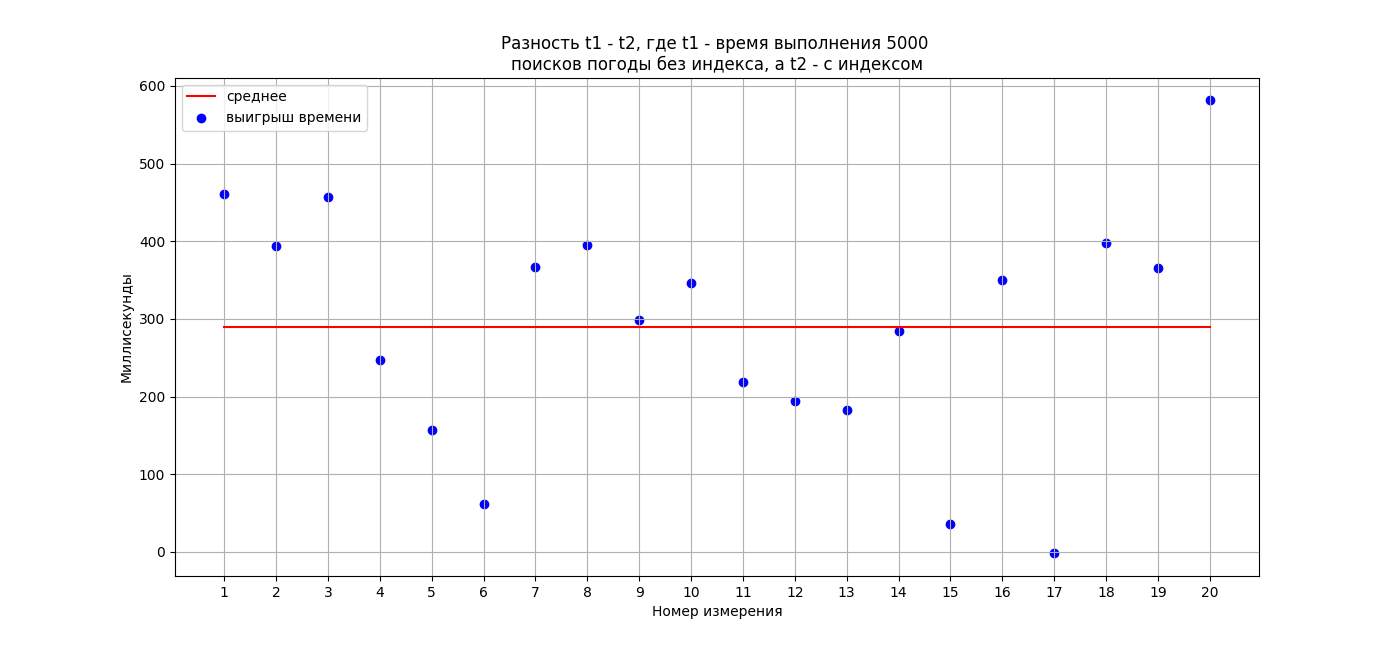
\includegraphics[width=\textwidth]{tools/img/plot1.png}
	\caption{
        Результаты измерений времени поиска погоды
    }
	\label{fig:plot1}
\end{figure}

\begin{figure}[H]
	\centering
	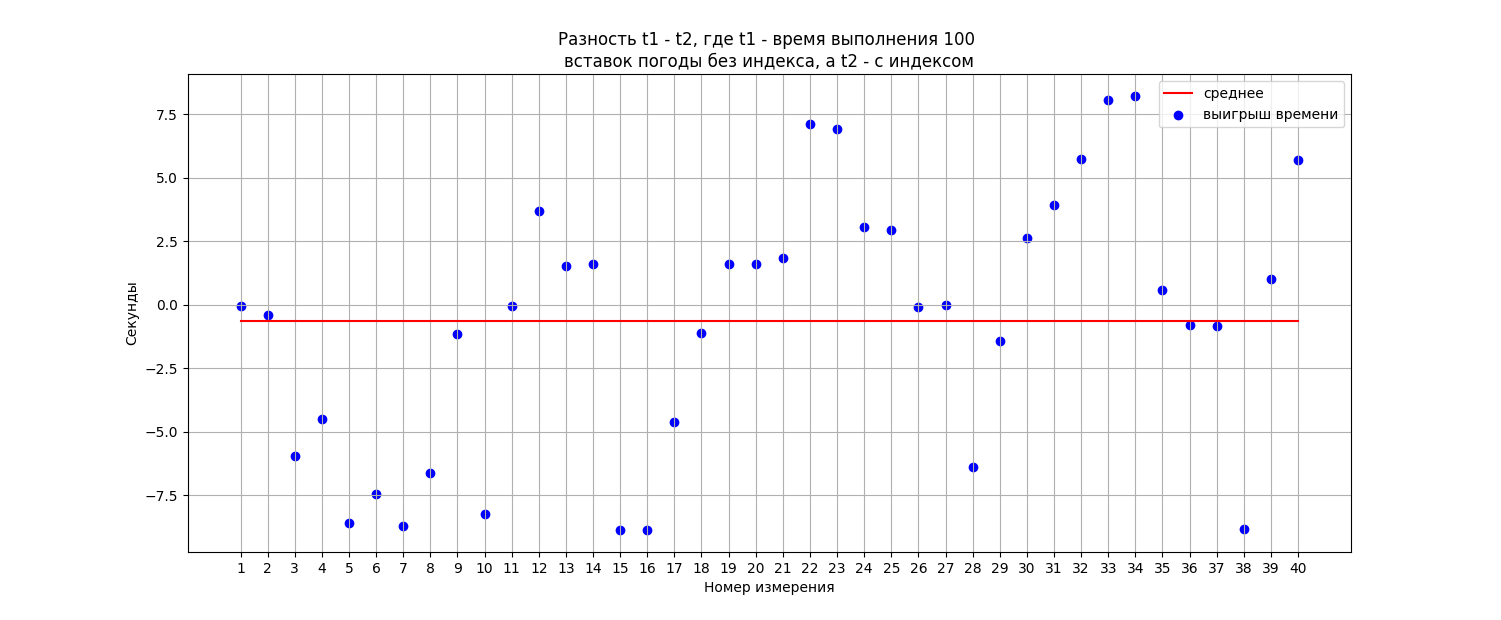
\includegraphics[width=\textwidth]{tools/img/plot2.png}
	\caption{
        Результаты измерений времени вставки массива погоды
    }
	\label{fig:plot2}
\end{figure}

\begin{figure}[H]
	\centering
	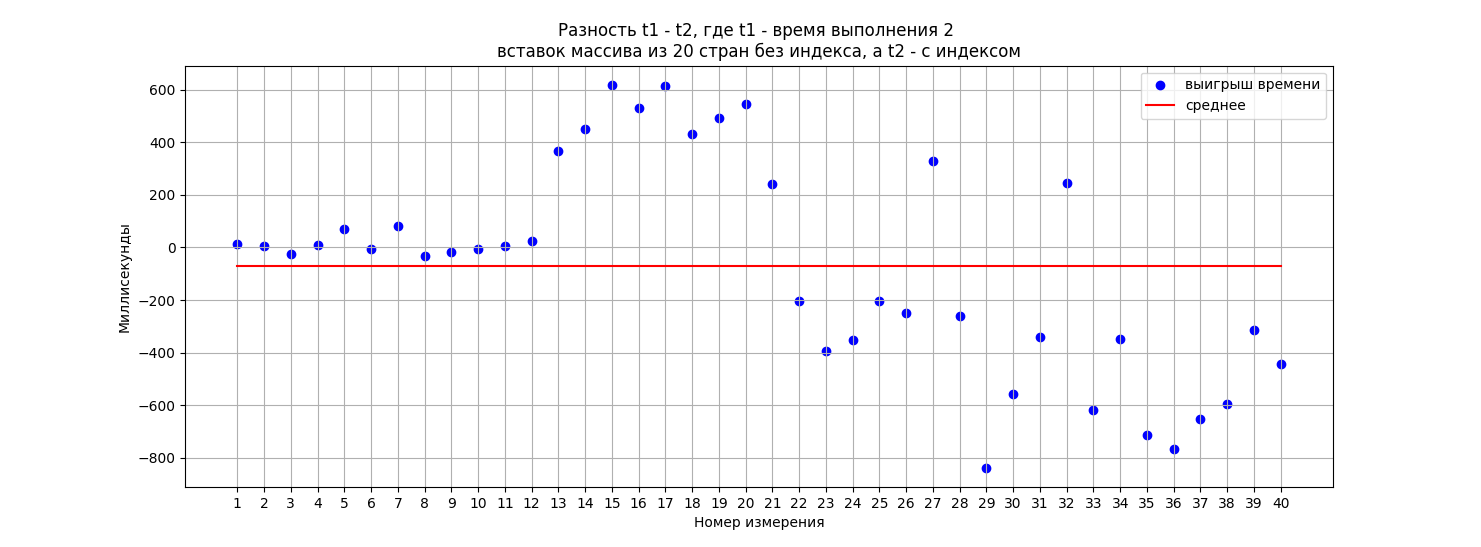
\includegraphics[width=\textwidth]{tools/img/plot3.png}
	\caption{
        Результаты измерений времени 2 вставок массива из 20 стран
    }
	\label{fig:plot3}
\end{figure}

\begin{figure}[H]
	\centering
	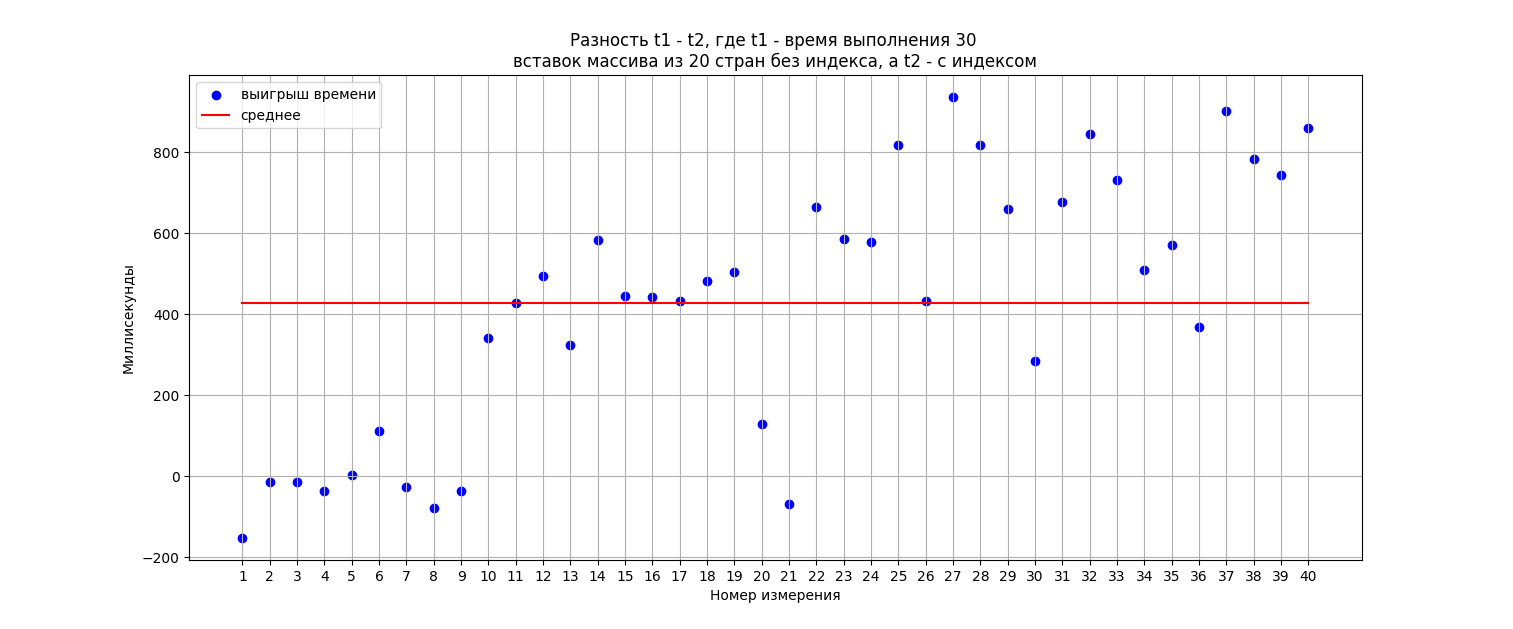
\includegraphics[width=\textwidth]{tools/img/plot4.png}
	\caption{
        Результаты измерений времени 30 вставок массива из 20 стран
    }
	\label{fig:plot4}
\end{figure}

Далее описано влияние индексов на временные характеристики прецедентов базы данных.
Поиск сущностей погоды погоды занял по времени на $3.8\%$ меньше, что составило приблизительно 300 миллисекунд.
Следовательно, индекс ускорил работу извлечения погоды из базы данных, как и ожидалось.
Вставка погоды после применения индекса начала выполняться дольше, но временные потери незначительны.
Именно это и ожидалось в результате применения индекса.
Таким образом, индекс для таблицы с погодой не оказывает значимого влияния на время выполнения прецедентов.
Поэтому его можно не использовать.

Индекс для таблицы со странами повлиял на время их вставки по различным сценариям.
Если в базу данных записываются страны, которые уже были в базе данных, то индекс ускоряет выполнение данного прецедента на $67\%$.
Это объясняется тем, что модуль базы данных перед вставкой каждой сущности проверяет, есть ли она в базе данных, а для этого необходимо выполнить поиск страны по имени.
Таким образом, индекс ускорил поиск страны и, следовательно, оптимизировал вставку дублирующихся стран.
Если же в базу данных записываются разные страны, то индекс повышает время вставки на приблизительно $20\%$.
Приложение, использующее базу данных чаще обновляет страны, чем вставляет новые.
Поэтому индекс для таблицы с городами следует применить.

Важным замечанием является то, что исходя из возможностей приложения пользователь не будет отправлять более 150 запросов к таблице с погодой и более 1 запроса на вставку стран или городов за 1 секунду.
Более того, кроме самих sql-запросов выполняется ещё и код приложения, содержащий сопоставимые по трудоёмкости операции.
Таким образом, пользователь не сможет заметить разницы между наличием и отсутствием любых индексов.
Следовательно, их использование а мобильном приложении под Android не обязательно.

\section*{Вывод из исследовательской части}
В данном разделе было продемонстрировано влияние реализованных индексов на время выподнения прецедентов базы данных.
В следствие этого сделан вывод об использовании индексов в базе данных приложения.